%% -----------------------------------------------------------------
%% This file uses UTF-8 encoding
%%
%% For compilation use following command:
%% latexmk -pdf -pvc -bibtex thesis
%%
%% -----------------------------------------------------------------
%%                                     _     _      
%%      _ __  _ __ ___  __ _ _ __ ___ | |__ | | ___ 
%%     | '_ \| '__/ _ \/ _` | '_ ` _ \| '_ \| |/ _ \
%%     | |_) | | |  __/ (_| | | | | | | |_) | |  __/
%%     | .__/|_|  \___|\__,_|_| |_| |_|_.__/|_|\___|
%%     |_|                                          
%%
%% -----------------------------------------------------------------

\documentclass{kithesis}

% Additional packages
\usepackage[main=slovak,english]{babel}

\usepackage{listings}
% Listings settings
% See for details: https://en.wikibooks.org/wiki/LaTeX/Source_Code_Listings
\lstset{
    basicstyle=\small\ttfamily,  % smaller typewriter font
    showstringspaces=false       % don't show spaces in string
}
\def\lstlistingname{Zdrojový kód}

% Variables
%\thesisspec{figures/thesisspec.png} 

\title{My thesis \br (the skeleton)}{Vizualizácia štruktúry genómu\br}

%\author{Janko Hraško}
\author[Bc.]{Oleksandr}{Korotetskyi}[]
\supervisor{doc. Ing. Ján Genči, PhD.} %veduci prace
\consultant{} %konzultant
%\college{University of Žilina}{Žilinská univerzita} %univerzita
%\faculty{Faculty of Electrical Engineering and informatics}{Fakulta elektrotechniky a informatiky} %fakulta
%\department{Department of Computers and Informatics}{Katedra počítačov a informatiky} %katedra
%\departmentacr{DCI}{KPI} % skratka katedry
%\thesis{Master thesis}{Diplomová práca} %typ prace
\submissiondate{28}{5}{2021}
%\fieldofstudy{9.2.1 Informatika}
%\studyprogramme{Informatika}
%\city{Košice} %mesto
\keywords{Programming, bioinformatics, data visualization, genome, covid-19}{Programovanie, bioinformatika, vizualizácia údajov, genóm, covid-19}
%\declaration{som nepodvadzal}

\abstract{%
    This bachelor thesis analyzes the general genome structure of different organisms (eukaryotes, prokaryotes and viruses) in order to understand the differences of various genomes and to come up with possible solutions for their visualization.
    Describes and compares some of popular existing programs that are designed for visualization of genome properties.
	As the next step, I perform 2D visualization and analysis of SARS-CoV-2 genome using some existing techniques and one developed by me.
    The results obtained during the visualization are verified and the code used to obtain them is composed into a stand-alone application.
}{%
    Bakalárska práca analyzuje všeobecnú štruktúru genómu rôznych organizmov (eukaryoty, prokaryoty a vírusy) s cieľom porozumieť rozdielom rôznych genómov a navrhnúť možné riešenia ich vizualizácie.
    Opisuje a porovnáva niektoré populárne existujúce programy, ktoré sú určené na vizualizáciu vlastnosti genómu.
    Zaobera sa 2D vizualizáciu a analýzu genómu SARS-CoV-2 nielen pomocou niektorých existujúcich, ale aj v práci vyvinutých techník.
    Výsledky dosiahnuté počas vizualizácie sa overuju a kód, použitý na ich získanie, prezentuje samostatnu aplikáciu.
}

\acknowledgment{Na tomto mieste by som rád poďakoval svojmu vedúcemu práce za jeho čas a odborné vedenie počas riešenia mojej záverečnej práce.

Rovnako by som sa rád poďakoval svojim rodičom a priateľom, najmä \textit{Adamovi Galuškovi} a \textit{Sultanu Shaimardanovi} za ich podporu a povzbudzovanie počas celého môjho štúdia.
    
V neposlednom rade by som sa rád poďakoval spoločnosti \textit{RedBull} a \textit{Ozzy Osbornovi} za energiu pri napísaní tejto práce.}

% if you want to work only on selected chapters
%\includeonly{chapters/analyza} %,chapters/synteza}

\thesisspec{chapters/ss.pdf}

% Load acronyms
\input{acronyms}


%% -----------------------------------------------------------------
%%          _                                       _   
%%       __| | ___   ___ _   _ _ __ ___   ___ _ __ | |_ 
%%      / _` |/ _ \ / __| | | | '_ ` _ \ / _ \ '_ \| __|
%%     | (_| | (_) | (__| |_| | | | | | |  __/ | | | |_ 
%%      \__,_|\___/ \___|\__,_|_| |_| |_|\___|_| |_|\__|
%%                                                      
%% -----------------------------------------------------------------

\begin{document}
%% Title page, abstract, declaration etc.:
\frontmatter{}

%% List of code listings, if you are using package minted
%\listoflistings

%\pagenumbering{arabic}

%% Chapters
% !TEX root = ../thesis.tex

\chaptermark{Úvod}
\phantomsection
\addcontentsline{toc}{chapter}{Úvod}

\chapter*{Úvod}

\par The order of DNA sequence and its variations are the very aspect which dictates the developmental processes of an organism, determines susceptibility to various diseases and uniquely identifies each creature. This area has always been on the periphery of the interests of scientific society, since the discovery in 1869 by Swiss-born biochemist Fredrich Miescher. For instance, The Human Genome Project (HGP) which started on October 1, 1990 and completed in April 2003 was one of the greatest feats of exploration in history of science. It was aimed at reading all the DNA sequences of our species, Homo sapiens. All in all, HGP introduced us the ability to read nature's complete genetic blueprint for building a human being. However, despite the successful completion of the project, a number of unknown DNA properties is still exists and demands the profound studying.

The knowledge of the genome structure has significantly increased in the past few decades thanks to the recent developments in the field of advanced analyzing techniques.\footnote{Askree, A.H., Yehuda, T., Smolikov, S., Gurevich, R., Hawk, J., Coker, C.,
Krauskopf, A., Kupiec, M., and McEachern, M.J. 2004. A genome-wide screen for Saccharomyces cerevisiae deletion mutants that affect telomere length. Proc. Natl. Acad. Sci. 101: 8658–8663.} The Sanger sequencing technology has been traditionally used to elucidate the DNA sequencing information since it was developed in the 1977th. However, it is capable of obtaining sequences of maximum length of 800 base pairs per one operation, which makes the sequencing process much longer and complicated. In spite of development of new sequencing techniques, some technology limits exist. For instance, the human genome in particular presents a number of major obstacles to correct read alignment, due to its size (3 GB) and complexity ( 48\% repetitive sequences), as do other plant plant and vertebrate genomes.

In addition, it is impossible to assemble the whole genome sequence of species using the data merely of one individual due to occurrence of the single nucleotide polymorphisms and mutations which affect the precise result. Several sequencing algorithms and searching methods were developed to deal with such issues which are the basis of the bioinformatics.\footnote{Danilevskaya, O.N., Arkhipova, I.R., Traverse, K.L., and Pardue, M.-L.
1997. Promoting in tandem: The promoter for telomere transposon HeT-A and implications for the evolution of retroviral LTRs. Cell 86: 647–655.} To be precise, the science was developed to deal with the next problems: assembling the complete nucleic acid sequence from the smaller parts, its comparison, analyzing and searching of similarities.

The usual eukaryotic genome consists not only of nuclear DNA, but also of DNA which is isolated from it and belongs to some organelles (mitochondrial mDNA, plastid DNA) that became a part of the cells in the evolution process. To identify key features and determine the exact genes at the complete DNA sequence, to distinguish the segments belonging to particular chromosomes it must visualized in some way. The whole genome might be visualized either as the two dimensional representation of the nucleotide sequence or as the 3D model of the spatial DNA or RNA architecture. The first way allows to analyze each gene and precisely identify each protein that it encodes and to trace the kinship of species, while the second way provides us with the possibility of understanding the inner cellular processes and the very interaction between different enzymes and nucleic acid from the chemical point of view. This work concerns mainly the first method of visualizing sequencing data. 

Although several DNA processing tools exist, the problem of representing different genome properties which might vary at various species, concerning either the number of particular genes or complete chromosomes (if they are present), remains still actual. Moreover, the processing of the genome and its visualization demand an efficient approach, concerning the size of data and computational capabilities of an average computer. This work aims at representing some key genome properties in such a way.

% !TEX root = ../thesis.tex

\chapter{Analytická časť}

In most eukaryotic and prokaryotic organisms the hereditary material is either linear double-stranded DNA 
(deoxyribonucleic acid) molecules or a circular double-stranded DNA molecule. However, some extracellular life forms, 
might use RNA (ribonucleic acid) as the building block for their genome. For instance, viruses have a genome composed of 
either single-stranded DNA, double-stranded DNA or RNA, depending on the type of a virus. Therefore, a genome itself, 
is the complete content of genetic information in an organism, or in other words, all the unique DNA or RNA sequences the organism possesses. 
\section{Nucleotides: the basic subunit of genome}

Both of DNA and RNA  are polymeric molecules, that are composed of linear chains of various combinations of four different subunits, called nucleotides. 
The nucleotide itself is the basic unit of the DNA and RNA molecules, the monomer, which, however, could be found in the cell not only as the bearer of the genetic information, 
but also as a carrier of energy used to power enzymatic reactions. A five-carbon-atom sugar, a phosphate group and a nitrogenous base are three distinct components which, 
combined together, make up the quite complex nucleotide molecule. The combination of sugar and base is called a nucleoside, while the phosphate-sugar-base is termed a nucleotide. 
The nucleotide bases can be either a single-ringed pyrimidine or a double-ringed purine. Dinucleotide, trinucleotide and polynucleotide are the terms corresponding to two, 
three or many nucleotides connected with each other respectively.

\begin{figure}[!ht]
	\centering
	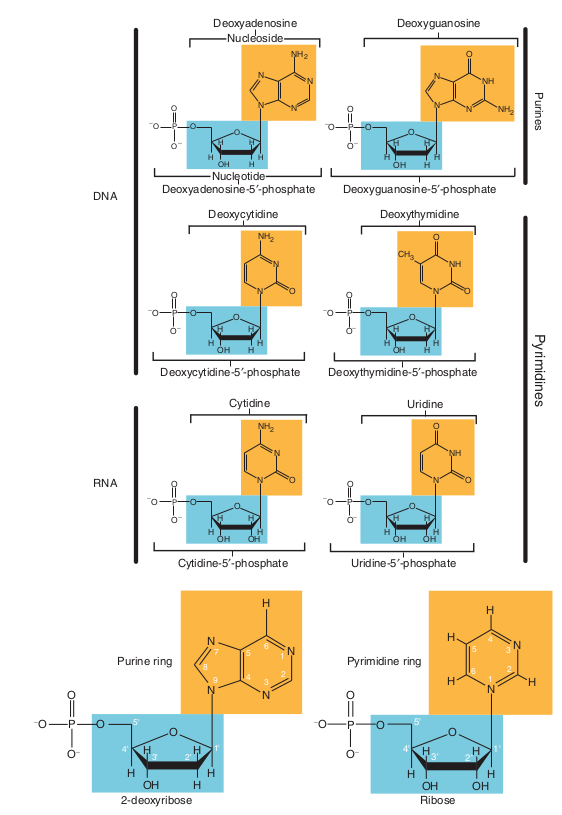
\includegraphics[width=.9\textwidth]{figures/bases}
	\caption{The structures of the pyrimidines and purines found in DNA and RNA. The sugar groups are highlighted in blue and the nitrogenous bases are highlighted in orange. 
	The atoms of the sugar are numbered from 1 to 5. The atoms of the purine ring are numbered from 1 to 9, 
	while those of the pyrimidine ring are numbered from 1 to 6. \label{o:latex_friendly_zone}}
\end{figure}

A nucleotide can be either a purine or pyrimidine. Guanine (G) and adenine (A) are the common purines for both of DNA and RNA; 
the pyrimidine called cytosine (C) is also present in both nucleic acids. However, the pyrimidine uracil (U) is limited only to RNA, 
being replaced with thymine (T) in DNA. There are merely two base-pair combinations that are permissible – A base-paired with T (U) and C base-paired with G. 
It happens due to the geometries of the nucleotide bases and relative positions of atoms which participate in the connection. 
This property makes two sequences of polynucleotides in helix complement. Discrete nucleotides are attached to each other through sugar–phosphate bonds 
that connect the phosphate group on the 5’ carbon of one nucleotide with the hydroxyl group on the 3’ carbon of another nucleotide. 
The base pairing between adenine and thymine (uracil) involves two hydrogen bonds, while between cytosine and guanine involves three hydrogen bonds.
\section{Nucleodic acid spatial stucture}

As the three-dimensional structure of a nucleotide is not completely rigid, it is possible for DNA to have various spatial architectures: 
A-form, B-form, Z-form and the circular one. The position of the base relatively to the five-carbon-atom sugar can be changed by a rotation 
around the N-glycosidic bond and, in this way, significantly affect the three dimensional configuration of the molecule and helix consequently.

\begin{table}[!ht]
	\caption{DNA double helix}\label{t:1}
	\smallskip
	\centering
	
	\begin{tabular}{ |p{3cm}||p{3cm}|p{3cm}|p{3cm}|  }
		\hline
		\multicolumn{4}{|c|}{Features of the different conformations of the DNA double helix} \\
		\hline
		Feature& B-DNA & A-DNA & Z-DNA\\
		\hline
		\hline
		Type of helix & Right-handed & Right-handed & Left-handed\\
		\hline
		Number of base pairs per turn & 10 & 11 & 12\\
		\hline
		Distance between base pairs (nm) & 0.34 & 0.29 & 0.37\\
		\hline
		Distance per complete turn (nm) & 3.4 & 3.2 & 4.5\\
		\hline
		Diameter (nm) & 2.37 & 2.55 & 1.84\\
		\hline
		Major groove & Wide, deep & Narrow, deep & Flat\\
		\hline
		Minor groove & Narrow, shallow & Wide shallow & Narrow, deep\\
		\hline
	\end{tabular}
\end{table}

Moreover, although usually single-stranded, some RNA sequences have the ability to form a double helix. 
However, double helix RNA is rare and has nothing in common with the genome itself, since only the 
single-stranded RNA molecules appear to participate in some genome related processes in the eukaryotic and prokaryotic organisms. 
Since circular DNA may exist in several forms including single-stranded c-DNA, intact double-stranded c-DNA (closed circles with both strands covalently linked), 
nicked ds-c-DNA (only one strand covalently linked) and “concatenated circles” their properties are not described in the attached table.

\section{Eukaryotic genome organization}

In eukaryotic cells nucleic acid is situated in a membrane-bound organelle called the nucleus.
The nuclear genome is split into a set of linear double-helix DNA molecules, each contained in a chromosome. 
No exceptions to this pattern are known: all eukaryotes that have been studied have at least two chromosomes and the DNA molecules are always linear. 
The only variability at this level of organization of eukaryotic genome is coherent with the number of chromosomes. 
Moreover, it appears, that biological features of an organism have no dependence on the number of chromosomes. 

\begin{figure}[!ht]
	\centering
	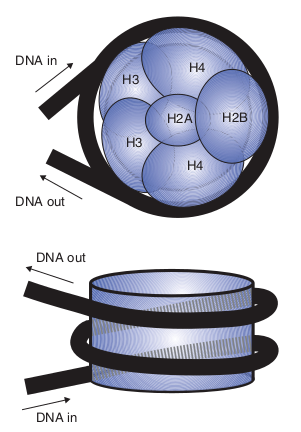
\includegraphics[width=.5\textwidth]{figures/nucleoDetailed}
	\caption{The nucleosome structure. H2A, H2B, H3 and H4 represent different types of histones. \label{o:latex_friendly_zone}}
\end{figure}

Despite the size of a nucleus (5-10 um), an overall length of DNA in the human cell is approximately 2.1m and can be packed inside the cell 
because of the method the nucleic acid is stored. The genetic material in viruses and bacteria consists of strings of DNA or RNA almost devoid of proteins. 
However, in eukaryotes, a substantial quantity of protein is associated with the DNA to form chromatin. At the lowest level, the DNA is organized by 
wrapping DNA strands around he proteins called histones, that contain a large amount of positively charged amino acids arginine and lysine. 
Those amino acids, and histones in general, play the crucial structural role, making it possible to bind the negative charged phosphate groups of the DNA nucleotides.

Averagely, the DNA rolled around the histones consists of 140-150 base pair, dependently on the species. Such a complex of DNA and histones is termed a nucleosome. 
These nucleosomes can be further coiled into increasingly larger coils up until forming chromosomes. However, tight coiling of DNA limits cells ability to access DNA and to process it.
Instead of being constantly coiled, the nucleic acid is usually found in a state called chromatin where some segments of acid are tightly reeled (heterochromatin), 
while other segments are entirely open (euchromatin). Euchromatin DNA is is highly accessible by the molecular complexes used by the cell and therefore is easier to manipulate with. 

The amount and extent of packing are determined by a sell, to control which sections of the genome can be expressed and which cannot. 
It affects cellular function and appears to be the predominant cause of differentiating cells type, while having the same DNA.

\begin{figure}[!ht]
	\centering
	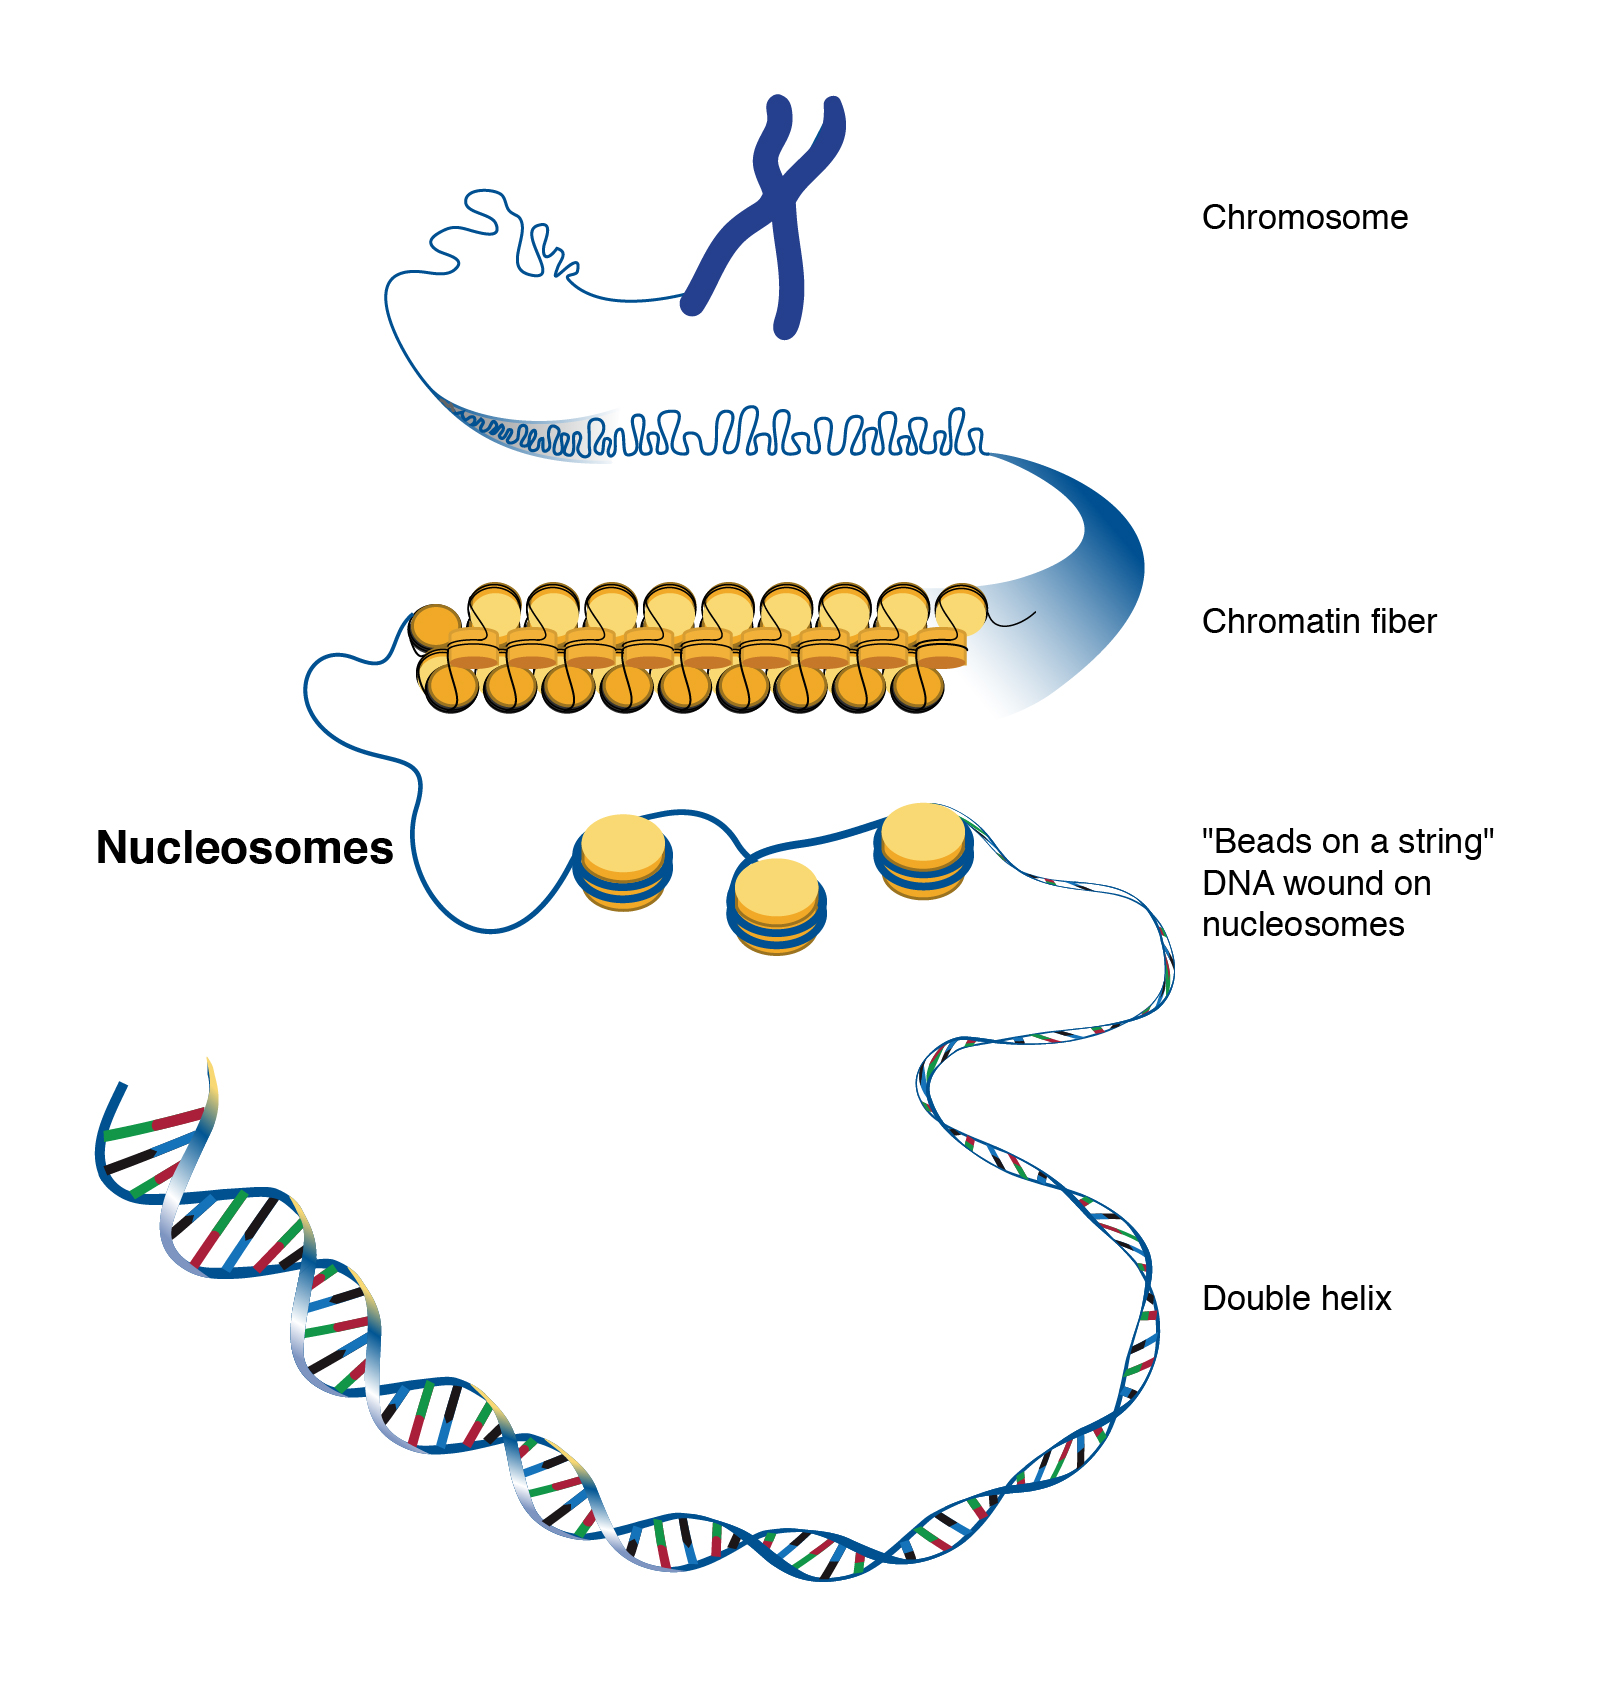
\includegraphics[width=.9\textwidth]{figures/nucleosome1}
	\caption{Ncleosomes as the part of a chromosome.\label{o:latex_friendly_zone}}
\end{figure}

\section{Prokaryotic genome organization}
Prokaryotic genomes are very different from eukaryotic ones, in particular with regard to the physical organization of the genome within the cell.
Although the word “chromosome” is used to describe the DNA–protein structures present in prokaryotic cells, this is a misnomer as this structure has few
similarities with a eukaryotic chromosome. 
The traditional view has been that in a typical prokaryote the genome is contained in a single, circular DNA molecule, 
localized within the nucleoid — the lightly staining region of the otherwise featureless prokaryotic cell. This is certainly true for E. coli and many of the other 
commonly studied bacteria.

Most of what we know about the organization of DNA in the nucleoid comes from studies of E. coli. The first feature to be recognized was that the circular
E. coli genome is supercoiled. Supercoiling occurs when additional turns are introduced into the DNA double helix (positive supercoiling) or if turns are
removed (negative supercoiling). With a linear molecule, the torsional stress introduced by over- or underwinding is immediately released by rotation of
the ends of the DNA molecule, but a circular molecule, having no ends, cannot reduce the strain in this way. Instead the circular molecule responds by
winding around itself to form a more compact structure. Supercoiling is therefore an ideal way to package a circular molecule into a small space. 
Evidence that supercoiling is involved in packaging the circular E.coli genome was first obtained in the 1970s from examination of isolated nucleoids, 
and subsequently confirmed as a feature of DNA in living cells in 1981. In E. coli, the supercoiling is thought to be generated and controlled by two enzymes, 
DNA gyrase and DNA topoisomerase I.

The E. coli genome, as described above, is a single, circular DNA molecule. This is also the case with the vast majority of bacterial and archaeal chromosomes 
that have been studied, but an increasing number of linear versions are being found. The first of these, for Borrelia burgdorferi, the organism that causes 
Lyme disease, was described in 1989, and during the following years similar discoveries were made for Streptomyces coelicolor and Agrobacterium tumefaciens. 
Linear molecules have free ends, which must be distinguishable from DNA breaks, so these chromosomes require terminal structures equivalent to the telomeres 
of eukaryotic chromosomes. In Borrelia and Agrobacterium, the real chromosome ends are distinguishable because a covalent linkage is formed 
between the 5` and 3` ends of the polynucleotides in the DNA double helix, and in Streptomyces the ends appear to be marked by special binding proteins.

\section{Genes: location and general structure}
Gene is a sequence of nucleotides in DNA or RNA that encodes the synthesis of a gene product, either RNA or protein that have distinctive features. At present we 
do not fully understand the nature of all of these specific features, and sequence inspection is therefore not a foolproof way of locating genes. 
Genes that code for proteins comprise open reading frames (ORFs) consisting of a series of codons that specify the amino acid sequence of the protein
that the gene codes for. The ORF begins with an initiation codon—usually (but not always) ATG — and ends with a termination codon: TAA, TAG, or TGA. 
Searching a DNA sequence for ORFs that begin with an ATG and end with a termination triplet is therefore one way of looking for genes. The analysis is 
complicated by the fact that each DNA sequence has six reading frames, three in one direction and three in the reverse direction on the complementary strand.

\begin{figure}[!ht]
	\centering
	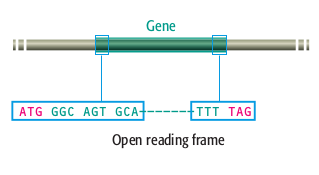
\includegraphics[width=.9\textwidth]{figures/ORF1.png}
	\caption{The
	first four and last two codons of the gene
	are shown. The first four codons specify
	methionine/initiation–glycine–serine–alanine,
	and the last two specify
	phenylalanine–termination.\label{o:latex_friendly_zone}}
\end{figure}


The key to the success of ORF scanning is the frequency with which termination codons appear in the DNA sequence. If the DNA has a random sequence
and a GC content of 50\% then each of the three termination codons — TAA, TAG, and TGA — will appear, on average, once every 64 bp. If the GC content 
is greater than 50\% then the termination codons, being AT – rich, will occur less frequently, but one will still be expected every 100–200 bp. This
means that random DNA should not show many ORFs longer than 50 codons in length, especially if the presence of a starting ATG triplet is used as part of
the definition of an ORF. Most genes, on the other hand, are longer than 50 codons: the average lengths are 317 codons for Escherichia coli, 483 codons
for Saccharomyces cerevisiae, and approximately 450 codons for humans. ORF scanning, in its simplest form, therefore takes a figure of, say, 100 codons
as the shortest length of a putative gene and records positive hits for all ORFs longer than this.


With bacterial genomes, simple ORF scanning is an effective way of locating most of the genes in a DNA sequence. shows a segment of the E. The real genes
in the sequence cannot be mistaken because they are much longer than 50 codons in length. With bacteria the analysis is further simplified by the fact
that the genes are very closely spaced and hence there is relatively little intergenic DNA in the genome (only 11\% for E. coli). If we assume that the 
real genes do not overlap, which is true for most bacterial genes, then it is only in the intergenic regions that there is a possibility of mistaking a short, 
spurious ORF for a real gene. So if the intergenic component of a genome is small, then there is a reduced chance of making mistakes in 
interpreting the results of a simple ORF scan. 

\begin{figure}[!ht]
	\centering
	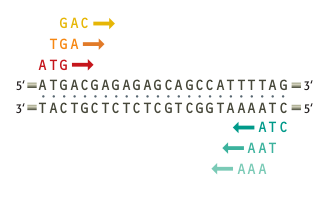
\includegraphics[width=.9\textwidth]{figures/ORF2.png}
	\caption{Both
	strands are read in the 5¢Æ3¢direction. Each
	strand has three reading frames, depending
	on which nucleotide is chosen as the
	starting position.\label{o:latex_friendly_zone}}
\end{figure}

Although ORF scans work well for bacterial genomes, they are less effective for locating genes in DNA sequences from higher eukaryotes. This is partly
because there is substantially more space between the real genes in a eukaryotic genome (for example, approximately 62\% of the human genome is intergenic), 
increasing the chances of finding spurious ORFs. But the main problem with the human genome and the genomes of higher eukaryotes in general is that their 
genes are often split by introns, and so do not appear as continuous ORFs in the DNA sequence. Many exons are shorter than 100 codons, some consisting of 
fewer than 50 codons, and continuing the reading frame into an intron usually leads to a termination sequence that appears to close the ORF. In other words, 
the genes of a higher eukaryote do not appear in the genome sequence as long ORFs, and simple ORF scanning cannot locate them.

Solving the problem posed by introns is the main challenge for bioinformaticists writing new software programs for ORF location. A good example of such software
is Glimmer. It uses machine learning for predicting the gene locations. Three modifications to the basic procedure for ORF scanning are usually adopted:

\begin{itemize}
	\item Codon bias is taken into account. “Codon bias” refers to the fact that not all codons are used equally frequently in the genes of a particular organism. 
	For example, leucine is specified by six codons in the genetic code (TTA, TTG, CTT, CTC, CTA, and CTG), but in human genes leucine is most frequently coded by 
	CTG and is only rarely specified by TTA or CTA. Similarly, of the four valine codons, human genes use GTG four times more frequently than GTA. The biological 
	reason for codon bias is not understood, but all organisms have a bias, which is different in different species. Real exons are expected to display the codon 
	bias whereas chance series of triplets do not. The codon bias of the organism being studied is therefore written into the ORF-scanning software.

	\item Exon–intron boundaries can be searched for as these have distinctive sequence features, although unfortunately the distinctiveness of these
	sequences is not so great as to make their location a trivial task. The sequence of the upstream exon–intron boundary is usually described as:
	5'–AGØGTAAGT–3' the arrow indicating the precise boundary point. However, only the “GT” immediately after the arrow is invariable: elsewhere in the sequence,
	nucleotides other than the ones shown are quite often found. In other words, the sequence is a consensus, by which we mean that the sequence shows the
	most frequent nucleotide at each position in all of the upstream exon–intron boundaries that are known, but that in any particular boundary sequence
	one or more of these positions might have a different nucleotide. The downstream intron–exon boundary is even less well defined: 5'–PyPyPyPyPyPyNCAGØ–3'
	where “Py” means one of the pyrimidine nucleotides (T or C) and “N” is any nucleotide. Simply searching for these consensus sequences will not
	locate more than a few exon–intron boundaries because most have sequences other than the ones shown. Writing software that takes account of the 
	known variables has proven difficult, and at present locating exon–intron boundaries by sequence analysis is a hit-and-miss affair.

	\item Upstream regulatory sequences can be used to locate the regions where genes begin. This is because these regulatory sequences, like exon–intron
	boundaries, have distinctive sequence features that they possess in order to carry out their role as recognition signals for the DNA-binding proteins
	involved in gene expression. Unfortunately, as with exon–intron boundaries, the regulatory sequences are variable, more so in eukaryotes than in prokaryotes, 
	and in eukaryotes not all genes have the same collection of regulatory sequences. Using these to locate genes is therefore problematic.
\end{itemize}

These three extensions of simple ORF scanning, despite their limitations, are generally applicable to the genomes of all higher eukaryotes. Additional
strategies are also possible with individual organisms, based on the special features of their genomes. For example, vertebrate genomes contain CpG
islands upstream of many genes, these being sequences of approximately 1kb in which the GC content is greater than the average for the genome as a
whole. Some 40\%–50\% of human genes are associated with an upstream CpG island. These sequences are distinctive and when one is located in vertebrate
DNA, a strong assumption can be made that a gene begins in the region immediately downstream.

ORF scanning is appropriate for protein-coding genes, but genes for functional RNAs such as rRNA and tRNA do not comprise open reading frames and hence 
will not be located by the methods described above. Functional RNA molecules do, however, have their own distinctive features, which can be used to aid 
their discovery in a genome sequence. The most important of these features is the ability to fold into a secondary structure, such as the cloverleaf 
adopted by tRNA molecules. These secondary structures are held together by base pairing not between two separate polynucleotides, as in the DNA double helix, 
but between different parts of the same polynucleotide—what we call intramolecular base pairing. In order for intramolecular base pairs to form, the
nucleotide sequences in the two parts of the molecule must be complementary, and to produce a complex structure such as the cloverleaf, the components of these 
pairs of complementary sequences must be arranged in a characteristic order within the RNA sequence. These features provide a wealth of information that 
can be used to locate tRNA genes in a genome sequence, and programs designed for this specific purpose are usually very successful.

As well as tRNAs, rRNAs and some of the small functional RNAs also adopt secondary structures that have sufficient complexity to enable their genes 
to be identified without too much difficulty. Other functional RNA genes are less easy to locate because the RNAs take up structures that involve 
relatively little base pairing or the base pairing is not in a regular pattern. Three approaches are being used for location of the genes for these RNAs:

\begin{figure}[!ht]
	\centering
	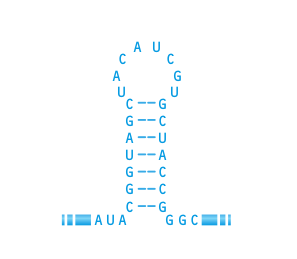
\includegraphics[width=.9\textwidth]{figures/rna.png}
	\caption{A typical RNA stem-loop
	structure.\label{o:latex_friendly_zone}}
\end{figure}

Most of the various software programs available for gene location by ORF scanning can identify up to 95\% of the coding regions in a eukaryotic
genome, but even the best ones tend to make frequent mistakes in their positioning of the exon–intron boundaries, and identification of spurious ORFs as
real genes is still a major problem. These limitations can be offset to a certain extent by the use of a homology search to test whether a series of triplets is a
real exon or a chance sequence. In this analysis the DNA databases are searched to determine if the test sequence is identical or similar to any genes
that have already been sequenced. Obviously if the test sequence is part of a gene that has already been sequenced by someone else then an identical
match will be found, but this is not the point of a homology search. Instead the intention is to determine if an entirely new sequence is similar to any
known genes because, if it is, then there is a chance that the test and match sequences are homologous, meaning that they represent genes that are evolutionarily related. 


\begin{itemize}
	\item Although some functional RNAs do not adopt complex secondary structures, most contain one or more stem-loops (or hairpins), which result
	from the simplest type of intramolecular base pairing. Programs that scan DNA sequences for such structures therefore identify regions where 
	functional RNA genes might be present. These programs incorporate thermodynamic rules that enable the stability of a stem-loop to be estimated, 
	taking into account features such as the size of the loop, the number of base pairs in the stem, and the proportion of G–C base pairs 
	(these being more stable than A–T pairs as they are held together by three rather than two hydrogen bonds). A putative stemloop structure 
	with an estimated stability above a chosen limit is considered a possible indicator of the presence of a functional RNA gene.

	\item As with protein-coding genes, a search can be made for regulatory sequences associated with genes for functional RNAs. These regulatory
	sequences are different to those for protein-coding genes, and may be present within a functional RNA gene as well as upstream of it.

	\item In compact genomes, attention is directed toward regions that remain after a comprehensive search for protein-coding genes. Often these
	“empty spaces” are not empty at all and a careful examination will reveal the presence of one or more functional RNA genes.
\end{itemize}

The main use of homology searching is to assign functions to newly discovered genes, and we will therefore return to it when we deal
with this aspect of genome analysis later in the chapter. The technique is also central to gene location because it enables tentative exon
sequences located by ORF scanning to be tested for functionality. If the tentative exon sequence gives one or more positive matches after a homology
search then it is probably a real exon, but if it gives no match then its authenticity must remain in doubt until it is assessed by one or other of 
the experiment-based gene location techniques.

A more precise version of homology searching is possible when genome sequences are available for two or more related species. Related species have
genomes that share similarities inherited from their common ancestor, overlaid with species-specific differences that have arisen since the species began
to evolve independently. Because of natural selection, the sequence similarities between related genomes are greatest within the genes and lowest in the 
intergenic regions. Therefore, when related genomes are compared, homologous genes are easily identified because they have high sequence similarity, 
and any ORF that does not have a clear homolog in the second genome can be discounted as almost certainly being a chance sequence and not a genuine gene. 
This type of analysis — called comparative genomics — is proving very valuable for locating genes in the Saccharomyces cerevisiae genome, as complete or partial
sequences are now available not only for this yeast but also for 16 other members of the Hemiascomycetes, including Saccharomyces paradoxus,
Saccharomyces mikatae, and Saccharomyces bayanus, the species most closely related to S. cerevisiae. Comparisons between these genomes have
confirmed the authenticity of a number of S. cerevisiae ORFs, and also enabled almost 500 putative ORFs to be removed from the S. cerevisiae catalog on the 
grounds that they have no equivalents in the related genomes. The analysis is made even more powerful by the synteny—conservation of gene
order—displayed by the genomes of these related yeasts. Although each genome has undergone its own species-specific rearrangements there are still
substantial regions where the gene order in the S. cerevisiae genome is the same as in one or more of the related genomes. This makes it very easy to
identify homologous genes but, more importantly, enables a spurious ORF, especially a short one, to be discarded with great confidence, because its
expected location in a related genome can be searched in detail to ensure that no equivalent is present.
% !TEX root = ../thesis.tex

\chapter{Syntetická časť}
\section{Existing Genome Browsers}
There are multiple genome browsers available. Some of them are
mentioned here:
\subsection{The UCSC Genome Browser}
It is one of the big players in genomic data visualization. The browser (Kent
et al. 2002) represents annotations as a series of horizontal tracks laid over
genome. Every track can be viewed in different modes such as dense, or
fully expanded or can be hidden. The user can go deeper on the dense track
25
to open it in full mode. There are many scales possible for the track display.
The lowest is a single chromosome and the highest scale is the sequence of
base pairs.
\subsection{The Galaxy Track Browser}
Visual Analytics is the science of using interactive visualizations in order
to support analytic reasoning. The Galaxy Track browser (J. Goecks et al.
2011) overcomes some of the shortcomings of other genomic browser by
using the concept of Visual Analytics. One of them is that the genome
browsers and their analysis tools are not integrated, this makes it tough
to change the parameter value of a tool so as to observe how the change
impacts the tool output in the browser. This can be done multiple times
to tune a tools parameter to obtain a desired output while staying in the
browser.
The Galaxy Track Browser gives freedom to the user to repeatedly change
the parameter’s value and rerun the tool multiple times. Morever, this can
be done interactively because the tool runs on the subset of the data that is
visible to the user. This is useful because users can receive feedback by manipulating data in real time. It provides a multi-resolution support model,
as well using the Galaxy framework provides visualization analysis easy
sharing of the results, all in just a web browser.
\subsection{Trackster}
Trackster (Jeremy Goecks et al. 2012) is another visual analysis environment
based on the Galaxy platform. It is targeted at analyzing the next generation sequencing data subsets by enabling the user to try different analysis
settings. All the outputs can be then visualized together interactively hence
making it easier to compare and inspect for the setting which works the
best. This also reduces the computational time by a large margin. It allows
dynamic integration of tools which are incorporated in the Galaxy framework. The firm coupling of tool settings and visualization enables rapid
tool parameter space exploration and dynamic data filtering.

\section{Parallel coordinates}
Parallel coordinate plots, in the context of gene expression data usually called profile
plots, are a method for visualizing high dimensional data. A point p ∈ R n is drawn on
n parallel axes by placing i-th vertex of a polyline on the position of the i-th axis that
represents the value of p i . A large number of points can be jointly visualized in parallel
coordinates. For interpreting the parallel coordinate plot, the order of the of the parallel
axes must be known. Parallel coordinate are used for a discrete number of dimensions,
like in discrete time series data. For this data, parallel coordinates are especially useful,
as the slope of the polylines is proportional to the difference between two adjacent time
points. The coordinates can also be spaced proportional to the distance between two
time points. Figure 3.3 shows an example of a parallel coordinate plot for time series
data.
Parallel coordinates were introduced in 1959 by Alfred Inselberg (a previous de-
scription of this concept was published by d’Ocagne in 1885) . Since then, par-
allel coordinates have been used in a multitude of applications. An influential paper
of Wegmann  demonstrated several use cases and interpretations. it included high-
dimensional geometric objects and cluster visualization, which is one of the most common
applications of parallel coordinates. For this purpose, color is used to indicate cluster
membership. Parallel coordinate plots can be extended by adding additional dimensions,
for example showing statistical properties of the points.
Plotting many points in parallel coordinates can lead to overplotting. To address
this problem, a number of dimension reduction methods have been suggested, e.g. .
Alternatively, clusters can be represented by centroids, leaving out all other points.
Using semitransparent lines gives a better overview of the density of lines in a plot. The
number of dimensions in a parallel coordinate plot is not generally limited. However, a
large number of dimensions might lead to tightly spaced coordinates, which can be hard
to read. For time series, an aspect ratio that causes the average slope of a line segment
to be 45° is considered optimal . This might lead to a trade-off between size and
readability.

\section{Visual Analytics}
While the roots of exploratory data analysis were based on manual calculations and
hand drawn graphics, possibly enhanced by desk calculators, modern methods greatly
increased the speed and handling of visualization and exploratory statistics. Interactivity
28
3.2. Visualization Plots
is a further important aspect made feasible by computer-based visualization. In the same
time, however, the size and complexity of datasets increased even faster then the analysis
tools were improved . New concepts for making sense of large, noisy and heterogenous
datasets are required. Visual analytics makes use of interactive visualization to support
human cognition to analyze and interpret data. The focus lies on the optimal support
of human cognition, which is considered a powerful tool. For this purpose, methods and
results from various scientific disciplines are integrated, including computer graphics,
psychology, cognitive sciences and design.
The overall process of visual analytics can be summarized by the visual analytics
mantra: “Analyse First - Show the Important - Zoom, Filter and Analyse Further - Details on Demand” . It names some of the tools and strategies used in visual analytics.
Analysis methods are used to prepare and filter the data to first visualize concentrating on important features . Visualizations are optimally maximizing data density and
should allow to easily identify patterns and relationships. Commonly tools used for EDA
are applied . Based on an existing visualization, refinements are interactively made:
zooming to get a view that is more coarse or fine, filtering to remove irrelevant items and
further analyses. Details on objects are shown interactively on demand. This process is
iteratively repeated. Each iteration is aimed at providing a useful visual representation
that allows the viewer to make more sense of the data.
As visual analytics is concerned with extremely large datasets, several challenges exist.
The limited space on visual media, especially screens calls for scalable visualizations (and
larger screens) . Analyzing high-throughput stream data can address data storage
problems. Another challenge is the analysis of heterogenous datasets, which arise in
many fields, including systems biology. Automatization of processes, decision support
and evaluation of existing processes are also fields of research in visual analytics.

\label{methodology}

\begin{thebibliography}{9}
    \bibitem{latexcompanion} 
    Stephan Symons, Christian Zipplies, Florian Battke, and Kay Nieselt.
    \textit{tephan Symons, Christian Zipplies, Florian Battke, and Kay Nieselt. Integrative
    Systems Biology Visualization with Mayday. Journal of Integrative Bioinformatics
    2010, 7:3}. 
    Addison-Wesley, Reading, Massachusetts, 1993.
    
    \bibitem{einstein} 
    Matthias Zschunke, Katrin Deubel, Stephan Symons, Janko Dietzsch, and Kay Nieselt. FAGE and VEGA
    \textit{A versatile algorithm and software for resequencing microarrays}. (German) 
    [\textit{On the electrodynamics of moving bodies}]. 
    Annalen der Physik, 322(10):891–921, 1905.

    \bibitem{einstein} 
    Florian Battke, Stephan Symons, Michael Piechotta, Philipp Bruns, Karin Zimmermann, and Kay Nieselt.
    \textit{Integrated    Expression Analysis}. (German) 
    [\textit{On the electrodynamics of moving bodies}]. 
    Annalen der Physik, 322(10):891–921, 1905.
    
    
% !TEX root = ../thesis.tex

\chapter{Vyhodnotenie}
\label{evaluation}
% !TEX root = ../thesis.tex

\chapter{Záver}
\label{summary}

% good linebraking of bibtex url
\setcounter{biburllcpenalty}{7000}
\setcounter{biburlucpenalty}{8000}

% %% The bibliography
\printbibliography[heading=bibintoc]

% \label{theend} % the last page of the thesis

% % List of acronyms
% \printglossary[type=\acronymtype,title={\acrlistname}]

% % Glossaries
% \printglossary

%% Appendix
% !TEX root = ../thesis.tex

\chapter*{Zoznam príloh}
\addcontentsline{toc}{chapter}{Zoznam príloh}

\begin{description}
    \item[Príloha A] Dokumentácia ku programu 
    \item[Príloha B] Vyvinutý program
    \item[Príloha C] CD médium -- záverečná práca v~elektronickéj podobe
\end{description}

\appendix
\renewcommand\chaptername{Príloha A}
% !TEX root = ../thesis.tex


\thispagestyle{empty}
	\begin{center}
		\vspace*{1cm}
		
		\textbf{\large Technicka Univerzita v Košiciach }
		
		\vspace{0.4cm}
		Fakulta elektrotechniky a informatiky
		
		\vspace{4.5cm}
		
		\textbf{\Large Dokumentácia k programu na vizualizáciu štruktúry genómu\\}
		\vspace{1.5cm}
		Príloha A k bakalárskej práci
		\vfill
		
		
		\vspace{2.8cm}
		
		{\raggedleft\vfill{%
		 		
			}\par}
		
		{\raggedright\vfill{%
				2021 \quad\quad\quad\quad\quad\quad\quad\quad\quad\quad\quad\quad\quad\quad\quad\quad\quad\quad\quad\quad\quad\quad\quad Oleksandr Korotetskyi
			}\par}
		
		
		
	\end{center}

\newpage
\rhead{Dokumentácia}
\addcontentsline{toc}{chapter}{Documentácia}
\subsubsection{\Large{Úvod}}
\addcontentsline{toc}{section}{Úvod}
Túto dokumentáciu možno považovať za používateľskú príručku k použitiu programu a ako systémovú príručku, ktorá popisuje funkčnosť a architektúru programu.

Dokumentácia je rozdelená na niekoľko častí, ktoré sa venujú zodpovedajúcim témam: inštalácia, scenáre spustenia a použitia, architektúra aplikácie.

\subsubsection{\Large{Inštalácia}}
\addcontentsline{toc}{section}{Inštalácia}
Aplikácia bola vyvinutá pre použitie hlavne na platformách Unix / Linux, a preto môže pokus o jej inštaláciu na platformu Windows viesť k neočakávanému správaniu programu.


\subsubsection{Python 3.8}
Aplikácia je napísaná v Pythone 3.8, a preto on je nevyhnutný pre použitie programu.
V systémoch založených na Debiane je možné ho nainštalovať pomocou nasledujúcich príkazov v termináli (štandardnóm príkazovóm riadku):
\begin{lstlisting}[language=bash]
  $ sudo apt-get update
  $ sudo apt-get install python3.8
\end{lstlisting}

Pre systémy založené na Fedore by sa mal použiť nasledujúci príkaz:
\begin{lstlisting}[language=bash]
  $ sudo dnf install python3
\end{lstlisting}


\subsubsection{Pip}
Ďalším krokom je inštalácia {\fontfamily{lmtt}\selectfont pip} (správca balíkov python), ktorý sa použije na inštaláciu ďalších závislostí.
Je to môžne urobiť pomocou nasledujúceho príkazu pre distribúcie založené na Debiane:
\begin{lstlisting}[language=bash]
  $ sudo apt-get install python3-pip
\end{lstlisting}

A pre systémy založené na Fedore musia byť použité:
\begin{lstlisting}[language=bash]
  $ curl "https://bootstrap.pypa.io/get-pip.py" -o "get-pip.py"
  $ python get-pip.py
\end{lstlisting}


\subsubsection{Knižnice}
Softvér pracuje na populárnych knižniciach, ktoré poskytujú používateľovi rozšírené funkcie pre sprácovanie genomov a ine účely.
Aby bolo možné aplikáciu používať, je potrebné nainštalovať nasledujúcich 12 balíkov:
{\fontfamily{lmtt}\selectfont
\begin{itemize}
    \item bio==0.4.1
    \item biopython==1.78
    \item matplotlib==3.4.2
    \item numpy==1.19.5
    \item pandas==1.2.4
    \item pillow==8.2.0
    \item pyparsing==2.4.7
    \item requests==2.25.1
    \item seaborn==0.11.1
    \item urllib3==1.26.4
    \item bcbio-gff
    \item dna\_features\_viewer
\end{itemize}
}

Úplný zoznam požadovaných balíkov sa nachádza v súbore \textbf{\fontfamily{lmtt}\selectfont requirements.txt}, ktorý je umiestnený v koreňovom adresári programu.

Samotnú inštaláciu knižníc je možné vykonať v termináli v koreňovom adresári programu pomocou jedného z nasledujúcich príkazov, ktoré sa môžu líšiť v závislosti od systému:
\begin{lstlisting}[language=bash]
  $ pip install -r requirements.txt
\end{lstlisting}
\begin{lstlisting}[language=bash]
  $ pip3 install -r requirements.txt
\end{lstlisting}

\addcontentsline{toc}{section}{Popis spustenia a činnosti aplikácie}
\subsubsection{\Large{Popis spustenia a  činnosti aplikácie}}
Tento vizualizačný nástroj podporuje dva režimy vykonávania: \textit {verbose} a \textit {quiet}.
Aplikácia v režime \textit{verbose} poskytuje používateľovi komentáre a prostredie na triviálnu interakciu, zatiaľ čo režim \textit{quit} je vhodnejší na účely rýchlejšej vizualizácie a automatizácie.

Oba režimy majú rovnaké funkcie, a preto sa líšia iba v tom, ako používateľ povie programovi, čo má robiť.
V režime \textit{verbose} používateľ komunikuje s programom prostredníctvom vstupu a výstupu konzoly, zatiaľ čo v režime \textit{quit} používa iba argumenty príkazového riadku.

Táto časť popisuje rôzne scenáre vykonávania programu v režime \textit{verbose} a sprevádzané príkazom na vykonanie rovnakej akcie iba pomocou argumentov príkazového riadku v režime \textit{quiet}.

Na spustenie aplikácie v režime \textit{verbose} by sa mal použiť jeden z nasledujúcich príkazov:
\begin{lstlisting}[language=bash]
  $ python3 Main.py
\end{lstlisting}
\begin{lstlisting}[language=bash]
  $ python3 Main.py -m v
\end{lstlisting}

Po spustení aplikácie sa objavi hlavné menu nástroja:
\begin{lstlisting}[language=bash]
  +----------------------------------+
  |--- Welcome to the Visualizer! ---|
  +----------------------------------+
  Choose the option: 
  1. Download SARS-CoV-2 genome sequence & associated files
  2. Plot sequence statistics
  3. Gates' visualization
  4. 2D Matrix visualization
  5. Improved 2D Matrix visualization
  6. Plot ORFs
  7. Compare genomes
  8. Exit
  Choice: 
\end{lstlisting}
Užívateľ je schopný voliť rôzné možnosti zadaním zodpovedajúceho im čísla.
Na ukončenie práci s nástrojem je potrebné stlačiť zadať „q“ pri hoci akom vstupe, na ktorý program čaká.


\subsubsection{Scenár 1}
Po výbere prvej možnosti sa v prípade úspechu zobrazia nasledujúce správy.
\begin{lstlisting}[language=bash]
  Necessary files are being downloaded...
  Done!
\end{lstlisting}
Všetky potrebné súbory (SARS-CoV-2.fasta a SARS-CoV-2.gb) sa úspešne stiahli.
Všetky ostatné súbory na vizualizáciu genómom musí používateľ pridať ručne do adresára {\fontfamily{lmtt}\selectfont data}.

\bigskip
Rovnaký scenár je možné vykonať v režime \textit{quiet} bez akýchkoľvek programových správ pomocou nasledujúceho príkazu:
\begin{lstlisting}[language=bash]
  $ python3 Main.py -m q -d
\end{lstlisting}


\subsubsection{Scenár 2}
Po výbere druhej možnosti program požiada používateľa, aby si vybral postupnosť z tých, ktoré sa nachádzajú v adresári {\fontfamily{lmtt}\selectfont data}.
\begin{lstlisting}[language=bash]
  Choose the sequence to plot the statistics of:
  1. alteromonas.fasta
  2. SARS-CoV-2.fasta
  3. ebola.fasta
  Choice: 2
\end{lstlisting}
Ďalším krokom je určenie intervalu, o ktorom sa musia štatistické údaje zobrazovať:
\begin{lstlisting}[language=bash]
  Specify the interval (0 for the entire genome)
  Start:	1223
  End:	0
\end{lstlisting}

Nuly predstavujú defaultné hodnoty, zatiaľ čo program vytvára tento výstup:
\begin{lstlisting}[language=bash]
  Frequencies of nucleotides on the interval [1223;29903]:
  A:	8626
  T:	9251
  G:	5577
  C:	5226
  Total:	28680
  GC-content on interval [1223;29903]:	0.3767%
\end{lstlisting}
Zobrazuju sa základné štatistické údaje analyzovanej sekvencie, ktoré by mohli byť užitočné.


\bigskip
Rovnaký scenár je možné vykonať v režime \textit{quiet} pomocou nasledujúceho príkazu:
\begin{lstlisting}[language=bash]
  $ python3 Main.py -m q -s --pos 1223 0
\end{lstlisting}



\subsubsection{Scenár 3}
Po výbere tretej možnosti program požiada používateľa, aby si vybral postupnosť z tých, ktoré sa nachádzajú v adresári {\fontfamily{lmtt}\selectfont data}.
\begin{lstlisting}[language=bash]
  Choose the sequence to visualize using Gates' method:
  1. alteromonas.fasta
  2. SARS-CoV-2.fasta
  3. ebola.fasta
  Choice: 3
\end{lstlisting}
Ďalším krokom je určenie intervalu sekvencie genómu, ktorý sa bude vizualizovať:
\begin{lstlisting}[language=bash]
  Specify the interval (0 for the entire genome)
  Start:	0
  End:	8000
  Done!
\end{lstlisting}

Generovaný obrázok je uložený v adresári {\fontfamily{lmtt}\selectfont out}.

\bigskip
Rovnaký scenár je možné vykonať v režime \textit{quiet} pomocou nasledujúceho príkazu:
\begin{lstlisting}[language=bash]
  $ python3 Main.py -m q -g ebola.fasta --pos 0 8000
\end{lstlisting}

\subsubsection{Scenár 4}
Po výbere štvrtej možnosti program požiada používateľa, aby si vybral postupnosť z tých, ktoré sa nachádzajú v adresári {\fontfamily{lmtt}\selectfont data}.
\begin{lstlisting}[language=bash]
  Choose the sequence to visualize using 2D Matrix method:
  1. alteromonas.fasta
  2. SARS-CoV-2.fasta
  3. ebola.fasta
  Choice: 3
  Done
\end{lstlisting}

Táto vizualizácia nepodporuje voľbu intervalu a vygenerovaný obrázok sa ukláda do adresára {\fontfamily{lmtt}\selectfont out}.

\bigskip
Rovnaký scenár je možné vykonať v režime \textit{quiet} pomocou nasledujúceho príkazu:
\begin{lstlisting}[language=bash]
  $ python3 Main.py -m q -x ebola.fasta
\end{lstlisting}

\subsubsection{Scenár 5}
Po výbere piatej možnosti program požiada používateľa, aby si vybral postupnosť z tých, ktoré sa nachádzajú v adresári {\fontfamily{lmtt}\selectfont data}.
\begin{lstlisting}[language=bash]
  Choose the sequence to visualize using 2D HMatrix method:
  1. alteromonas.fasta
  2. SARS-CoV-2.fasta
  3. ebola.fasta
  Choice: 2
\end{lstlisting}

Ďalším krokom je zadavánie veľkosti vytvoreného obrázka a po ňom program vygeneruje nasledujúci výstup:
\begin{lstlisting}[language=bash]
  Specify the size of image (preferably a power of 2, >= 512):
  Size (px):	2048
  seed: f9fa11164acc370f5c187a286c25dcffe0b93363c68ce5d658d83e
  w, h: 1024.0, 512.0
  w, h: 256.0, 256.0
  opacity: 50%
  w, h: 128.0, 64.0
  opacity: 37%
  w, h: 32.0, 32.0
  opacity: 25%
  w, h: 16.0, 8.0
  opacity: 15%
  w, h: 4.0, 4.0
  opacity: 9%
  w, h: 2.0, 1.0
  opacity: 5%
  Done
\end{lstlisting}

Vygenerovaný obrázok sa ukláda do adresára {\fontfamily{lmtt}\selectfont out}.

\bigskip
Rovnaký scenár je možné vykonať v režime \textit{quiet} bez výstupu konzoly pomocou nasledujúceho príkazu:
\begin{lstlisting}[language=bash]
  $ python3 Main.py -m q -i ebola.fasta -S 2048
\end{lstlisting}



\subsubsection{Scenár 6}
Po výbere šiestej možnosti program požiada používateľa, aby si vybral anotačný súbor genómu, ktorý sa má použiť, z tých, ktoré sa nachádzajú v adresári {\fontfamily{lmtt}\selectfont data}.
\begin{lstlisting}[language=bash]
  Choose the annotation file to visualize ORFs:
  1. ebola.gb
  2. SARS-CoV-2.gbk
  Choice: 2
  Done  
\end{lstlisting}
Vygenerovaný obrázok sa úspešne ulkláda do adresára {\fontfamily{lmtt}\selectfont out}.

\bigskip
Rovnaký scenár je možné vykonať v režime \textit{quiet} bez výstupu konzoly pomocou nasledujúceho príkazu:
\begin{lstlisting}[language=bash]
  $ python3 Main.py -m q -o SARS-CoV-2.gbk
\end{lstlisting}



\subsubsection{Scenár 7}
Po výbere siedmej možnosti program požiada používateľa, aby vybral sekvencie genómu na porovnanie so sekvenciami, ktoré sa nachádzajú v adresári {\fontfamily{lmtt}\selectfont data}.
\begin{lstlisting}[language=bash]
  Choose the first sequence to compare:
  1. alteromonas.fasta
  2. SARS-CoV-2.fasta
  3. ebola.fasta
  Choice: 2
  Choose the second sequence to compare:
  1. alteromonas.fasta
  2. SARS-CoV-2.fasta
  3. ebola.fasta
  Choice: 3
  Similarity (%): 72  
\end{lstlisting}
Po samotnom porovnaní program zadá percento podobnosti.

\bigskip
Rovnaký scenár je možné vykonať v režime \textit{quiet} bez výstupu konzoly pomocou nasledujúceho príkazu:
\begin{lstlisting}[language=bash]
  $ python3 Main.py -m q -c SARS-CoV-2.fasta ebola.fasta
\end{lstlisting}


\subsubsection{Použitie režimu Quiet}
Pre ziskanie dokladnéj informácií o režime \textit{quiet}, používateľ môže zadať nasledujúci príkaz:
\begin{lstlisting}[language=bash]
  $ python3 Main.py -h
\end{lstlisting}

Tento príkaz zobrazuje všetky podporované argumenty príkazového riadku:
\begin{lstlisting}[language=bash]
usage: Main.py [-h] [-m {q,v}] [-d] [-g GATES] [-o ORF] [-s] 
               [-x MATRIX] [-i HASH] [-c COMP COMP] [-S SIZE]
               [-p POS POS] [-a] [-n NAME]

optional arguments:
  -h, --help            show this help message and exit
  -m {q,v}, --mode {q,v}
                        Execution mode: quiet / verbose
  -d, --download        Download SARS-CoV-2 genome associated 
                        files
  -g GATES, --gates GATES
                        Perform Gates' visualization. Parameter
                        is an input sequence filename
  -o ORF, --orf ORF     Plot ORFs of the genome. Parameter is 
                        an input sequence filename
  -s, --stat            Obtain genome statistical data including
                        the distribution of nucleotides 
                        and a GC-content
  -x MATRIX, --matrix MATRIX
                        Plot the nucleotide sequence into a 2D 
                        matrix. Parameter is the input sequence 
                        filename
  -i HASH, --hmatrix HASH
                        Plot the nucleotide sequense into Hashed
                        2D matrix. Parameter is input sequence 
                        filename
  -c COMP COMP, --compare COMP COMP
                        Compare specified genome sequences using 
                        the pairwise2 algorithm
  -S SIZE, --size SIZE  Size of the picture side in pixels
  -p POS POS, --pos POS POS
                        Start and end positions of the nucleotide 
                        sequence to perform an action (0 for default)
  -a, --all             Perform all possible actions but comparison
                        in the default mode
  -n NAME, --name NAME  Input sequnce filename
\end{lstlisting}


\rhead{Dokumentácia}
\subsubsection{\Large{Architektúra aplikácie}}
\addcontentsline{toc}{section}{Architektúra aplikácie}
Vyvinutý program predstavuje samostatnú konzolovú aplikáciu, ktorá sa skladá z 8 modulov umiestnených v koreňovom adresári programu.
Obsah adresára je uvedený nižšie:
\textbf{\fontfamily{lmtt}\selectfont
\begin{itemize}
    \item Main.py
    \item Comparison.py
    \item GatesVisualization.py
    \item MatrixVisualization.py
    \item HMatrixVisualization.py
    \item ORFPlotter.py
    \item SeqCollector.py
    \item StatGenerator.py
    \item requirements.txt
\end{itemize}
}

Počas chodu programu sa vytvárajú dva ďalšie adresáre so súbormi, ak neexistujú: \textbf{\fontfamily{lmtt}\selectfont data} a \textbf{\fontfamily{lmtt}\selectfont out}.

Prvý adresár obsahuje stiahnuté sekvencie a program ho považuje za zdrojový adresár všetkých sekvencií genómu a súborov anotácií genómu, s ktorými program pracuje.
Preto, aby bolo možné vizualizovať a pracovať s vlastnými genómami, ich súbory musia byť vložené do adresára \textbf{\fontfamily{lmtt}\selectfont data}.

Druhý slúži na uloženie všetkých výstupných obrázkov formátu {\fontfamily{lmtt}\selectfont .png}, ktoré program vytvorí.
Preto, aby si užívateľ mohol pozrieť vykonané vizualizácie, musí ich vyhľadať v adresári \textbf{\fontfamily{lmtt}\selectfont out}.

\rhead{Dokumentácia}
\subsubsection{Modules description}
\textbf{\fontfamily{lmtt}\selectfont Main.py} je hlavný modul programu, ktorý je zodpovedný za použitie zvyšných modulov na vykonanie zadanej úlohy.
Zaoberá sa vstupom a výstupom z konzoly, navrhuje dostupné metódy vizualizácie a získava podrobnosti potrebné na ich výkon.
Obsahuje nasledujúce funkcie:
\begin{itemize}
  \item \textbf{\fontfamily{lmtt}\selectfont verifyArgs()} -- overuje a kontroluje argumenty príkazového riadku, ak je program spustený v režime \textit{quiet}. Ak sa vyskytne chyba, program sa zastaví.
  \item \textbf{\fontfamily{lmtt}\selectfont welcomeBanner()} -- ak je zapnutý režim \textit{verbose}, zobrazí "uvítací banner".
  \item \textbf{\fontfamily{lmtt}\selectfont mainMenu()} -- ak je režim \textit{verbose} zapnutý, zobrazí hlavné menu aplikácie a požiada používateľa, aby vybral možnosť pokračovania; skontroluje vstup používateľa. Vráti číslo vybratého scenára.
  \item \textbf{\fontfamily{lmtt}\selectfont vObtainFiles(msg)} -- ak je zapnutý režim \textit{verbose}, vypíše všetky súbory vo formáte {\fontfamily{lmtt}\selectfont FASTA} a požiada používateľa, aby si jeden vybral. Parameter {\fontfamily{lmtt}\selectfont msg} predstavuje správu, ktorá sa má zobraziť. Vráti názov vybraného súboru, ak je prítomný, v opačnom prípade sa zobrazí chybové hlásenie a funkcia vráti hodnotu {\fontfamily{lmtt}\selectfont None}.
  \item \textbf{\fontfamily{lmtt}\selectfont vObtainFiles2(msg)} -- ak je zapnutý režim \textit{verbose}, vypíše všetky súbory vo formáte {\fontfamily{lmtt}\selectfont GenBank} a požiada používateľa, aby si jeden vybral. Parameter {\fontfamily{lmtt}\selectfont msg} predstavuje správu, ktorá sa má zobraziť. Vráti názov vybraného súboru, ak je prítomný, v opačnom prípade sa zobrazí chybové hlásenie a funkcia vráti hodnotu {\fontfamily{lmtt}\selectfont None}.
  \item \textbf{\fontfamily{lmtt}\selectfont vObtainInterval()} -- ak je režim \textit{verbose} zapnutý, požiada používateľa, aby určil interval sekvencie genómu, na ktorom má vykonať akciu. Vráti pozície {\fontfamily{lmtt}\selectfont start} a {\fontfamily{lmtt}\selectfont end} po ich overení.
  \item \textbf{\fontfamily{lmtt}\selectfont vObtainSize()} -- ak je zapnutý režim \textit{verbose}, požiada používateľa, aby určil veľkosť pre vygenerovanie štvorcového obrázku. Vráti veľkosť strany obrázka v pixeloch.
  \item \textbf{\fontfamily{lmtt}\selectfont main()} -- vykoná hlavný cyclus programu a určuje, ktorú akciu má vykonať podľa argumentov príkazového riadku a vstupu používateľa. V režime \textit{quiet} končí program po vykonaní akcie, zatiaľ čo v režime \textit{verbose} znova zobrazí hlavné menu aplikácie.
\end{itemize}



\textbf{\fontfamily{lmtt}\selectfont SeqCollector.py} je zodpovedný za stiahnutie všetkých požadovaných sekvencií a súborov anotácií z databázy NCBI pre vizualizáciu genómu SARS-CoV-2.
V tejto chvíli nepodporuje sťahovanie súborov spojených s inými genómami.
Obsahuje nasledujúce funkcie:
\begin{itemize}
  \item \textbf{\fontfamily{lmtt}\selectfont downloadFiles()} -- vytvorí adresár {\fontfamily{lmtt}\selectfont data}, ak neexistuje, a stiahne (vyžaduje sa internetové pripojenie) sekvenciu genómu a anotačné súbory SARS-CoV-2.
\end{itemize}



\textbf{\fontfamily{lmtt}\selectfont StatGenerator.py} získava štatistické údaje, ako je obsah GC a distribúcia nukleotidov / aminokyselín.
Užívateľ si môže zvoliť oblasť genómu, ktorá sa má štatisticky analyzovať.
Obsahuje nasledujúce funkcie:
\begin{itemize}
  \item \textbf{\fontfamily{lmtt}\selectfont getStats(filename, mode, start, end)} -- overuje typ {\fontfamily{lmtt}\selectfont filename}. Overuje {\fontfamily{lmtt}\selectfont start} a {\fontfamily{lmtt}\selectfont end} pozície. Funkcia zastaví vykonávanie programu v chybových prípadoch a zobrazí príslušné chybové hlásenie. Vypisuje štatistické údaje o zadanom intervale sekvencie genómu a poskytne používateľovi ďalšie komentáre v režime \textit{verbose}.
\end{itemize}



\textbf{\fontfamily{lmtt}\selectfont GatesVisualization.py} vykonáva vizualizáciu pomocou Gatesovej metódy do súboru {\fontfamily{lmtt}\selectfont -Gates.png} .
Užívateľ je schopný zvoliť oblasť genómu ktorú chce vizualizovať.
Obsahuje nasledujúce funkcie:
\begin{itemize}
  \item \textbf{\fontfamily{lmtt}\selectfont visualize(filename, mode, start, end)} -- overuje typ {\fontfamily{lmtt}\selectfont filename}. Overuje {\fontfamily{lmtt}\selectfont start} a {\fontfamily{lmtt}\selectfont end} pozície. Funkcia zastaví vykonávanie programu v chybových prípadoch a zobrazí príslušné chybové hlásenie. Vykonáva Gatesovu vizualizáciu určeného intervalu sekvencie genómu.
  \item \textbf{\fontfamily{lmtt}\selectfont save(outFileName, image)} -- vytvorí adresár {\fontfamily{lmtt}\selectfont out} ak neexistuje, a uloží vygenerovaný obrázok {\fontfamily{lmtt}\selectfont outFileName} do adresára {\fontfamily{lmtt}\selectfont out}.
\end{itemize}



\textbf{\fontfamily{lmtt}\selectfont MatrixVisualization.py} kreslí zvolený genóm pomocou generácie 2D matice do súboru {\fontfamily{lmtt}\selectfont -Matrix.png} .
Veľkosť výstupného obrázka sa počíta automaticky.
Obsahuje nasledujúce funkcie:
\begin{itemize}
  \item \textbf{\fontfamily{lmtt}\selectfont visualize(filename)} -- overuje typ {\fontfamily{lmtt}\selectfont filename}. Funkcia zastaví vykonávanie programu v chybových prípadoch a zobrazí príslušné chybové hlásenie. Vykoná vizualizáciu sekvencie špecifikovaného genómu jeho vykreslením do 2D matice.
\end{itemize}



\textbf{\fontfamily{lmtt}\selectfont HMatrixVisualization.py} kreslí genóm do 2D matice vybranej veľkosti pomocou algoritmu hash funkcie do súboru {\fontfamily{lmtt}\selectfont -Hmatrix.png} .
Veľkosť výstupného obrázka môže byť zádana používateľom.
Obsahuje nasledujúce funkcie:
\begin{itemize}
  \item \textbf{\fontfamily{lmtt}\selectfont save(outFileName, image)} -- vytvorí adresár {\fontfamily{lmtt}\selectfont out}, ak neexistuje, a uloží vygenerovaný obrázok{\fontfamily{lmtt}\selectfont outFileName} do adresára {\fontfamily{lmtt}\selectfont out}.
  \item \textbf{\fontfamily{lmtt}\selectfont drawLayer(imgSize, depth, mode)} -- kreslí farébne bloky na základe {\fontfamily{lmtt}\selectfont getRandomColor()} vo veľkosti {\fontfamily{lmtt}\selectfont getBlockSize(imgSize, depth)} pre jednotlivé vrstvy. Vráti obrázok aktuálnej vrstvy. Poskytuje používateľovi ďalšie komentáre v režime \textit{verbose}.
  \item \textbf{\fontfamily{lmtt}\selectfont getHash(filename)} -- počíta hash sekvencie genómu {\fontfamily{lmtt}\selectfont filename}.
  \item \textbf{\fontfamily{lmtt}\selectfont getRandomColor()} -- vráti n-ticu náhodných hodnôt farieb vo formáte RGB.
  \item \textbf{\fontfamily{lmtt}\selectfont getBlockSize(imgSize, depth)} -- počíta a vracia {\fontfamily{lmtt}\selectfont width} a {\fontfamily{lmtt}\selectfont height} podľa {\fontfamily{lmtt}\selectfont imgSize} a {\fontfamily{lmtt}\selectfont depth}. S každou iteráciou cyklu sa každá strana bloku delí na polovicu alebo na štvrtiny, v závislosti od {\fontfamily{lmtt}\selectfont depth}.
  \item \textbf{\fontfamily{lmtt}\selectfont visualize(filename, mode, ssize)} -- skontroluje typ {\fontfamily{lmtt}\selectfont filename} a zastaví vykonávanie programu v prípade chýb. Vykonáva 2D Hashed Matrix vizualizáciu určenej sekvencie genómu rekurzívnym spôsobom. Upraví {\fontfamily{lmtt}\selectfont seed} na generovanie náhodných čísel na základe funkcie {\fontfamily{lmtt}\selectfont getHash(filename)}. Zlúči vrstvy veľkosti {\fontfamily{lmtt}\selectfont size} vytvorené funkciou {\fontfamily{lmtt}\selectfont drawLayer(size, depth, mode)} v závislosti od definovanej {\fontfamily{lmtt}\selectfont opacity}. Poskytuje používateľovi ďalšie komentáre v režime \textit{verbose}.
\end{itemize}



\textbf{\fontfamily{lmtt}\selectfont ORFPlotter.py} generuje obraz distribúcie ORF a pomeru obsahu GC v genóme do súboru {\fontfamily{lmtt}\selectfont -ORFs.png} .
Obsahuje nasledujúce funkcie:
\begin{itemize}
  \item \textbf{\fontfamily{lmtt}\selectfont visualize(filename)} -- overuje príponu {\fontfamily{lmtt}\selectfont filname}. Funkcia zastaví vykonávanie programu v chybových prípadoch a zobrazí príslušné chybové hlásenie. Vykoná vizualizáciu súboru s anotáciami určeného genómu zobrazením ORF.
  \item \textbf{\fontfamily{lmtt}\selectfont save(outFileName, plt)} -- vytvorí adresár {\fontfamily{lmtt}\selectfont out} ak neexistuje, a uloží vygenerovaný plot {\fontfamily{lmtt}\selectfont plt} do adresára {\fontfamily{lmtt}\selectfont out}.
\end{itemize}

\textbf{\fontfamily{lmtt}\selectfont Comparison.py} vykonáva porovnanie zvolenych genómov. Percento podobnosti sa získa na základe algoritmu pairwise2.
Obsahuje nasledujúce funkcie:
\begin{itemize}
  \item \textbf{\fontfamily{lmtt}\selectfont compare(filename1, filename2, mode)} -- overuje typy súborov {\fontfamily{lmtt}\selectfont filename1} a {\fontfamily{lmtt}\selectfont filename2} a zastaví vykonávanie programu v prípade chyby a poskytne používateľovi príslušnú správu. Vykonáva porovnanie vybraných sekvencií genómu pomocou algoritmu pairwise2. Poskytuje používateľovi ďalšie komentáre v režime \textit{verbose}.
\end{itemize}

\subsubsection{\Large{Záver}}
\addcontentsline{toc}{section}{Záver}
Táto dokumentácia predstavuje komplexný prehľad softvéru, ktorý bol vyvinutý počas bakalárskej práce „Vizualizácia štruktúry genómu“.

Aplikácia pracuje v dvoch možných režimoch a umožňuje používateľovi vizualizovať a analyzovať genómy rôznych organizmov pomocou sady vopred určených techník.

Inštalácia, vykonanie, technické aspekty a scenáre použitia boli podrobne popísané v príslušných častiach.

Na záver by sa ďalšie vylepšenia mohli zamerať na aplikovánie objektovo-orientovanej paradigmy programovania na architektúru programu a na pridanie nových funkcionalít.



% zivotopis autora
%\curriculumvitae\protect
%Táto časť\/ je nepovinná. Autor tu môže uviesť\/ svoje biografické
%údaje, údaje o~záujmoch, účasti na~projektoch, účasti na~súťažiach,
%získané ocenenia, zahraničné pobyty na~praxi, domácu prax, publikácie
%a~pod.

\end{document}
